
\section{Проблем проналаска суме у бинарном стаблу}

\subsection{Опис проблема}
Cтабло је граф који је повезан и који нема циклуса.
Бинарно стабло је усмерено стабло у коме сваки чвор, почевши од коренског чвора, има 0, 1 или 2 деце-чворова. Дететом чвора називамо чвор на кога неки други чвор показује.
Родитељем чвора називамо чвор који на неки други чвор показује. Листом називамо чвор који има 0 деце.

У примеру испод, плавом је приказана једна путања која даје тражену суму 22.

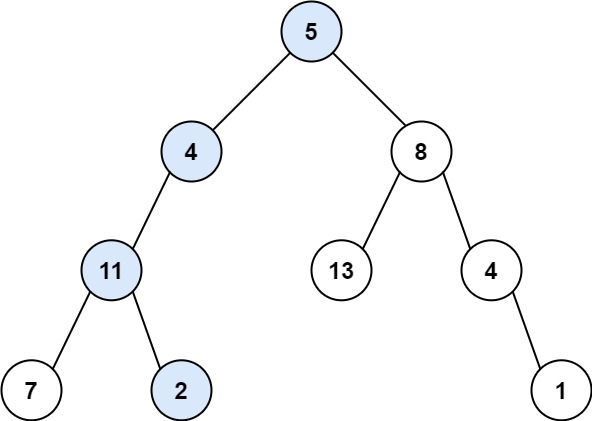
\includegraphics[scale = 0.4]{pathsum1.jpg}

За проблем су дата два улаза: стабло и тражена сума, док је тражен један излаз: булова променљива чија је тачност еквивалентна чињеници да је решење пронађено, односно
да за дати граф постоји путања од корена до листа која даје тражену суму.

% \begin{table}[]
%     \begin{tabular}{ll}
%         & Улаз           \\
%     1 & Бинарно стабло \\
%     2 & Тражена сума  
%     \end{tabular}
% \end{table}

% \begin{table}[]
%     \begin{tabular}{ll}
%       & Излаз             \\
%     1 & Булова променљива
%     \end{tabular}
% \end{table}

\subsection{Секвенцијално решење проблема}

Најчешће секвенцијално решење проблема своди се на обилазак графа по дубини (енг. \textit{depth first search}, DFS).
Овакво решење има асимптотску временску сложеност извршавања $O(n)$ gde $n$ представља величину улаза tj. број елемената у графу.

Програмски код за секвенцијално решење дато је у листингу \ref{code:sekvencijalno}. Напомена: изостављен је део кода за учитавање и креирање графа.

\begin{listing}
\inputminted{c}{kodovi/basic.c}
\caption{Имплементација секвенцијалног решења у језику \texttt{C}}
\label{code:sekvencijalno}
\end{listing}

\pagebreak
